\section{Introduction}
\label{sec:intro}

This work contains a collection of applications of the 
Discrete Gauss-Bonnet theorem.
I hope that the number of applications continues to grow,
please share any that you feel
ought to  be included\footnote{\text{bradleymccoy@montana.edu}}.
Here we emphasize the \emph{discrete} Gauss-Bonnet
theorem and most of our applications are related to algorithms. 
Several applications of the continuous version of the theorem
are given in \cite{doc76}, for applications of the Gauss-Bonnet 
theorem in physics see \cite{tirado-physics-apps}.

The Discrete Gauss-Bonnet theorem states that the sum of curvature
of a manifold at each point is $2\pi$ times the Euler characteristic.
The theorem is a bridge between topological
and geometric information, see \figref{bridge}. 
This bridge can be traversed in both directions.
That is, if one has geometric information one can deduce topological information and
if one has topological information one can deduce geometric information.


\begin{figure}[htb]
\centering
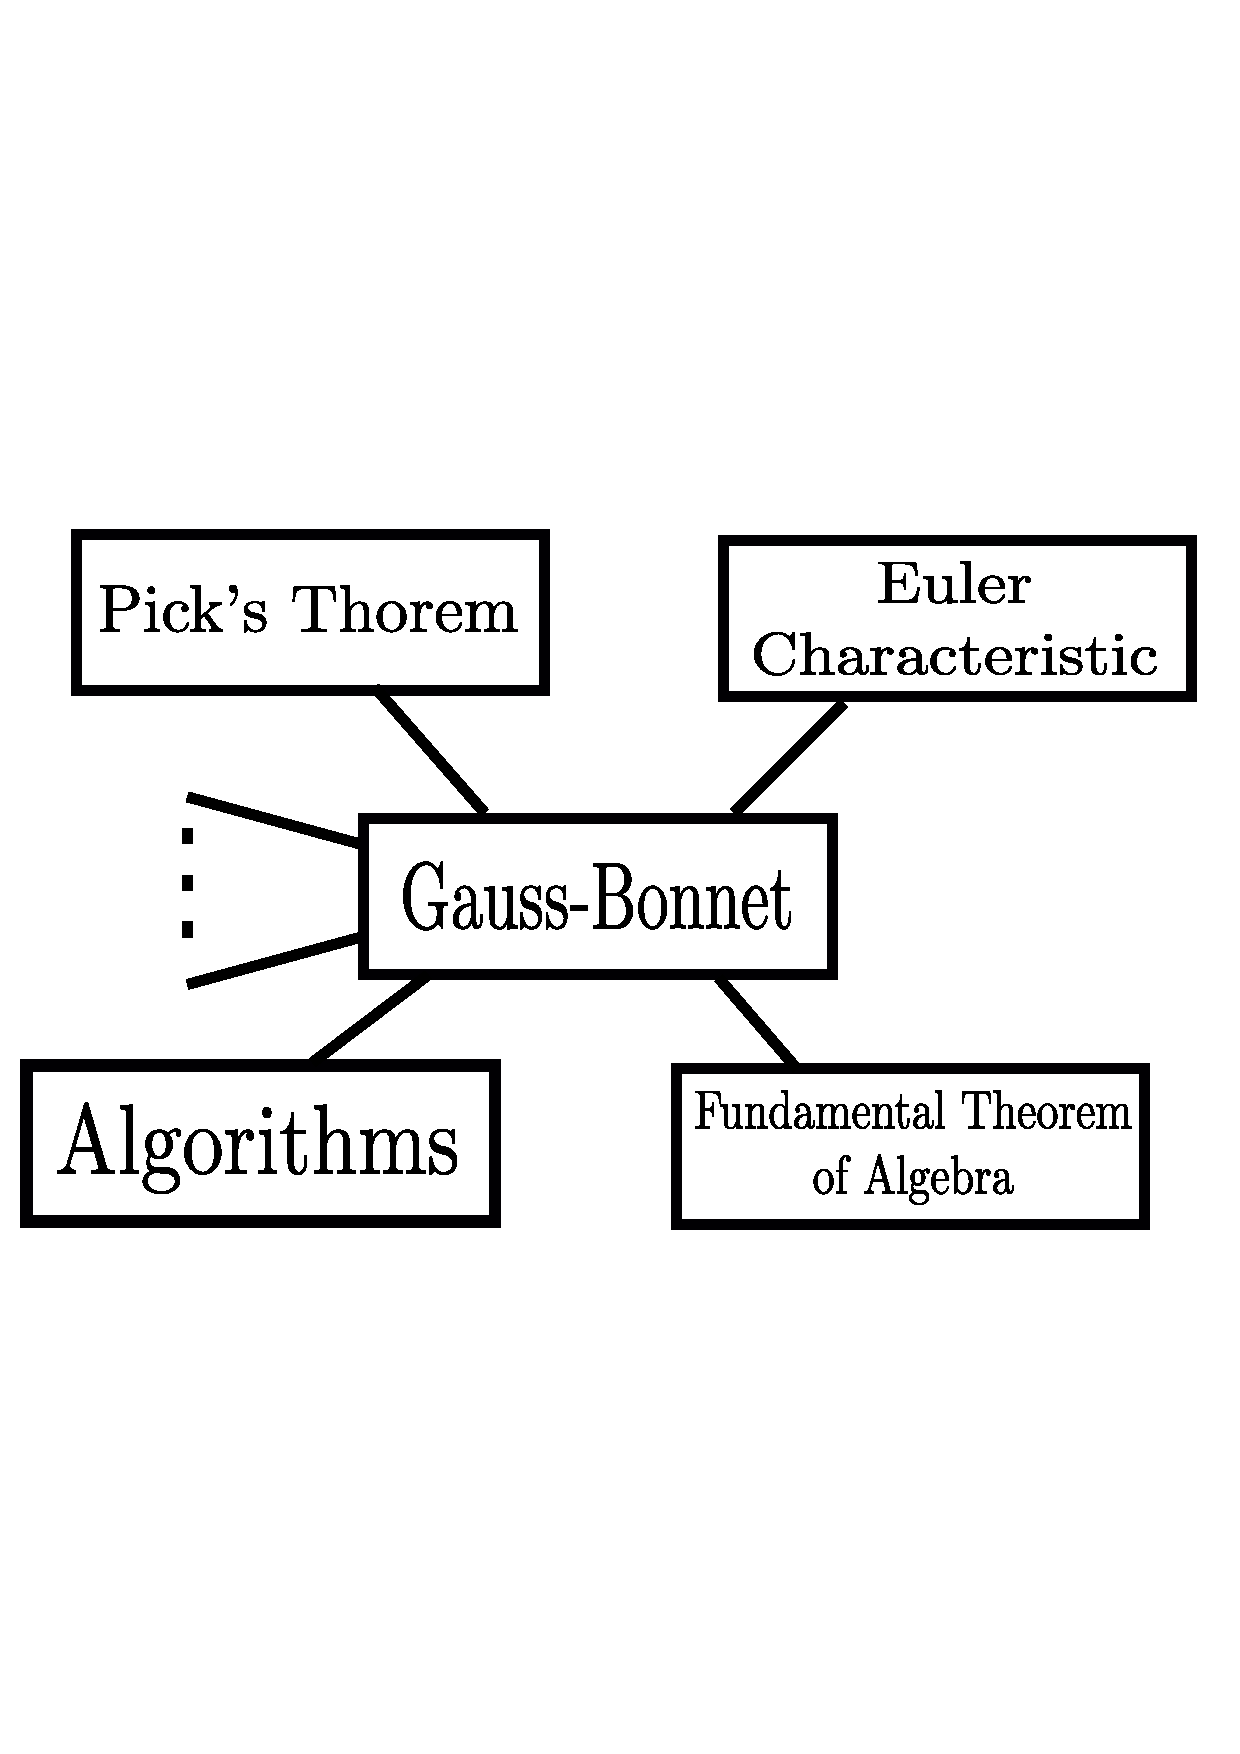
\includegraphics[width=.3\textwidth]{curvature/bridge}
\caption{The Gauss-Bonnet theorem allowing bi-directional traffic
between geometry and topology.}
\label{fig:bridge}
\end{figure}

This work is inspired by Matou\v{s}ek's book \emph{Using the Borsuk-Ulam Theorem}
\cite{jm08}.
Matou\v{s}ek states that a theorem is a great theorem if there are
\begin{enumerate}[(1)]
\item several different equivalent versions,
\item many different proofs,
\item a host of extensions and generalizations, and
\item numerous interesting applications.
\end{enumerate}

By this standard, the Gauss-Bonnet theorem is a great theorem.
For (1), will state several different versions of the theorem throughout this paper.
As for (2), several proofs exist.
For (3), one example of a generalization is the celebrated Atiyah–Singer index 
theorem \cite{atiyah_index_1963}.
This work is dedicated to (4).

This paper is organized as follows:
in \secref{background} we introduce definitions and notation that will be used
throughout the paper. We then state and prove the theorem.
In each subsection of \secref{applications}, we present an application of the theorem.
In general, the sections containing applications are ordered from simpler to more technical,
and are independent.


